\documentclass[sigconf,review,anonymous]{acmart}
\settopmatter{printacmref=false}
\acmConference{}{}{}
\acmDOI{}
\acmISBN{}
\setcopyright{none}
\ccsdesc[500]{Security and privacy~Distributed systems security}
\ccsdesc[300]{Computing methodologies~Distributed algorithms}
\renewcommand\footnotetextcopyrightpermission[1]{}
\usepackage{booktabs}
\usepackage{graphicx}
\usepackage{xcolor}
\usepackage{url}
\usepackage{tikz}
\usetikzlibrary{positioning}
\definecolor{papergray}{gray}{0.35}
\title{Beyond Checkpoint Repair: Lifecycle Evaluation of Backdoor Defenses in Federated Learning}
\author{Anonymous Author(s)}
\begin{document}
\begin{abstract}
Endpoint attack success alone does not characterize exposure during continued federated training. A deployed federated model is exposed to a sequence of accepted updates, and a repair that lowers attack success at one checkpoint may be rejected by a private gate, undone by later training, or appear effective only because evaluation occurs immediately after a scheduled repair. We evaluate this lifecycle effect across five seeds in a 400-trajectory main comparison and a 200-trajectory baseline comparison, with 100 rounds per trajectory on FEMNIST writer cohorts held out from earlier experiments and freshly partitioned Fashion-MNIST. The main comparison crosses clean training, attacker-stop poisoning, and continuous poisoning with quorum aggregation, update clipping, periodic validation-based repair, clean fine-tuning, and an activation-based Fine-Pruning adaptation, with private and diagnostic forced admission for the repair methods. We report attack success over committed rounds, post-stop exposure, endpoint attack success, clean accuracy, and admission decisions. For the patch trigger, periodic repair reduces attacker-stop endpoint attack success on FEMNIST from 86.15\% for quorum to 4.74\%, but the mean attack success after the attacker stops remains 44.81\%. Under continuous poisoning, its mean post-onset attack success is 94.62\% and endpoint attack success is 7.35\%. Our Fine-Pruning adaptation also leaves substantial temporal exposure. These results show why endpoint measurements do not establish lifecycle protection and why private admission must be evaluated together with subsequent training. A companion comparison with NAD-style repair and coordinate-median aggregation shows that these outcomes depend on the trigger, dataset, and admission policy.\end{abstract}
\keywords{federated learning, backdoor attacks, model repair, private validation, lifecycle evaluation}
\maketitle
\fancyhead[LE,RO]{}

\section{Introduction}
Federated learning (FL) trains a shared model from client updates without collecting the clients' raw training data. The same update interface lets a compromised client influence the shared model. Backdoor attacks exploit this interface by making inputs with a trigger produce an attacker-selected label while preserving ordinary accuracy. Many defenses therefore screen updates, clip their norms, or repair a global model with a small clean reference set. Clean accuracy and attack success rate (ASR) at the end of training summarize the final model, but do not specify exposure during training.

That endpoint view omits the deployment process. A model may be served after every committed round. A repair may be admitted by a private validator panel that sees a skewed and limited sample. Future honest and malicious updates then move the model away from the repaired checkpoint. Conversely, a scheduled repair can make an endpoint look safe even when most preceding rounds exposed users to a backdoor. These cases create different security questions: whether a candidate is safe at a checkpoint, whether the admission rule commits it, and how much attack exposure occurs over the subsequent trajectory.

This paper examines repair, admission, and subsequent training within a common experimental design. We compare update-level defenses and model-repair methods under attacker-stop and continuous poisoning, measuring the models committed throughout training. The central hypothesis is that endpoint attack success can substantially understate exposure across a deployment horizon when the endpoint coincides with scheduled repair.

Periodic repair lowers final checkpoint ASR after the attacker stops, while residual exposure over the post-stop horizon remains much larger. Continued poisoning sustains high temporal exposure even when scheduled repair lowers endpoint ASR. Fine-Pruning reduces endpoint ASR on Fashion-MNIST, but leaves high temporal exposure on FEMNIST; forced admission also reduces clean accuracy.

\paragraph{Contributions.} We make four contributions.
\begin{itemize}
\item We define a lifecycle evaluation that separates candidate repair, private admission, and post-admission training, with ASR measured over committed rounds.
\item We compare eight policies in 400 trajectories and four policies in a companion 200-trajectory comparison across two datasets, five seeds, two trigger families, and two poisoning schedules.
\item We quantify the endpoint-temporal gap and the interaction between private admission and continued poisoning.
\item We compare NAD-style repair and coordinate-median aggregation to distinguish admission effects from update-level robustness and clean-utility trade-offs.
\end{itemize}

\section{Background and Related Work}
Backdoor attacks in FL were established as a model-poisoning threat in which a malicious client replaces or scales an update to implant a trigger \cite{bagdasaryan2020how}. Neurotoxin showed that a backdoor can remain effective after the attacker stops submitting poisoned updates, motivating an explicit stopped-attacker condition \cite{zhang2022neurotoxin}. FLTrust and related robust aggregation methods use a trusted reference signal or update statistics to limit malicious influence \cite{cao2021fltrust}. Client hardening and filtering approaches such as FLIP operate at the client or update level, while teacher-guided repair methods such as NAD use clean examples to remove a learned backdoor \cite{wang2022flip,li2021nad}. Fine-Pruning was originally proposed for centralized networks and removes dormant neurons before fine-tuning \cite{liu2018finepruning}; we adapt it to the shared small CNN.

Private client feedback and admission have been studied in BaFFLe and CrowdGuard, which make client behavior or feedback part of model selection \cite{fu2020baffle,zhang2022crowdguard}. These works motivate our separation of a repair candidate from the decision that commits it. The distinction matters because a private panel is a measurement instrument with its own data support and error modes.

Recent work reinforces the need for adversarial evaluation beyond a single attack and checkpoint. The ACM CCS 2024 study of distributed backdoors in federated graph learning reports high attack success under several topologies and evaluates a certified defense \cite{yang2024distributed}. An ACM Transactions on Privacy and Security study examines backdoors in peer-to-peer FL under non-IID data and limited adversarial visibility \cite{syros2024p2p}. In 2025, MARS targets adaptive backdoors that respond to whether an update is accepted \cite{wan2025mars}, while SDBA studies durable backdoors in NLP FL \cite{li2025sdba}. A 2025 survey groups attack and defense evaluation criteria and identifies persistence and cross-setting validity as open problems \cite{li2025survey}. Prodigal, published in 2026, studies poisoning transfer in robust aggregation and reports experiments across several image datasets \cite{liu2026prodigal}. Persistence after attacker withdrawal is therefore an established evaluation concern. Our contribution is an empirical comparison that jointly records candidate outcomes, private admission, scheduled repair phase, and subsequent committed-round exposure.

\section{Threat Model and Lifecycle}

\begin{figure*}[t]
\centering
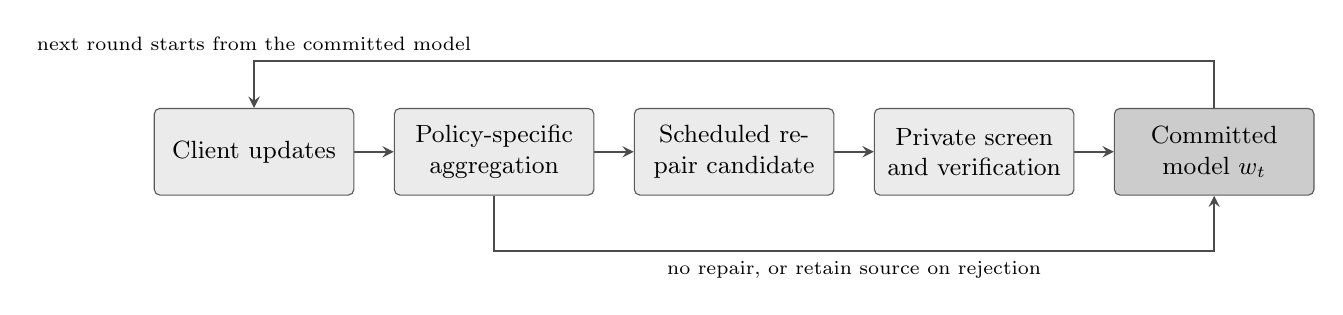
\begin{tikzpicture}[node distance=5mm,box/.style={draw=black!65,fill=black!8,rounded corners=2pt,align=center,font=\small,minimum height=11mm,text width=23mm},arr/.style={->,>=stealth,thick,draw=black!70}]
\node[box] (updates) {Client updates};
\node[box,right=of updates] (aggregate) {Policy-specific aggregation};
\node[box,right=of aggregate] (repair) {Scheduled repair candidate};
\node[box,right=of repair] (admit) {Private screen and verification};
\node[box,right=of admit,fill=black!20] (commit) {Committed model $w_t$};
\draw[arr] (updates)--(aggregate);
\draw[arr] (aggregate)--(repair);
\draw[arr] (repair)--(admit);
\draw[arr] (admit)-- (commit);
\draw[arr] (aggregate.south)--++(0,-.7) -| node[pos=.25,below,font=\scriptsize]{no repair, or retain source on rejection} (commit.south);
\draw[arr] (commit.north)--++(0,.6)-| node[pos=.5,above,font=\scriptsize]{next round starts from the committed model} (updates.north);
\end{tikzpicture}
\caption{Model lifecycle. Repair and admission use disjoint private client groups. Held-out test measurements follow the commit decision and have no feedback path into the policy. Non-repair baselines follow the direct aggregation-to-commit path.}
\Description{Five stages connect updates, aggregation, scheduled repair, private admission, and the committed model. A bypass retains the source when repair is absent or rejected, and a feedback arrow starts the next training round.}
\label{fig:lifecycle}
\end{figure*}

We consider synchronous cross-device FL with 50 clients and 40\% participation per round. The server aggregates client updates and may execute a repair at rounds 25, 50, 75, and 100. Fifteen clients (30\%) are malicious in attacked conditions. The attacker targets label 0 and scales each malicious update by the participant-to-attacker ratio, $20/6$, before defense-specific processing. In the attacker-stop condition, poisoning is applied in rounds 11--50 and then stops. In the continuous condition, poisoning continues through round 100. Providers and validators are honest; corrupted repair providers, adaptive attackers, and collusion are outside the evaluated threat model.

Figure~\ref{fig:lifecycle} distinguishes model construction, admission, and subsequent training. The deployed state at round $t$ is the model that passes the controller and is committed. For a trigger set $T$, we report the committed attack success rate $A_t$. The primary security metric is the seed-level mean over rounds 11--100, with two secondary summaries: mean $A_t$ over rounds 51--100 for attacker-stop runs and $A_{100}$. A low $A_{100}$ therefore does not imply low exposure over the trajectory.

Each repair produces a candidate from the current model. Separate private screening and verification panels compare clean behavior and loss under synthetic transformations. The private arm commits only when the shared admission rule passes; the forced arm commits the candidate for diagnosis and is not a deployable policy. We record the candidate, decision, committed model, and parent model at every intervention.

\paragraph{Training adversaries and honest panel behavior.}
Malicious training roles and malicious validation behavior are separate experimental factors. Clients assigned to poisoning can be sampled for repair or validation, but execute those roles honestly in this study. The allocation excludes current training participants; it does not filter clients using attacker identities. Under an alternative model in which every malicious training client also corrupts validation, a five-client sample from all 50 clients would contain at least one such client with probability
\begin{equation}
 1-\frac{\binom{35}{5}}{\binom{50}{5}}=84.68\%.
\end{equation}
For the actual nonparticipant pool, six of the 15 malicious clients have participated, leaving nine among 30 clients. The analogous probability is $1-\binom{21}{5}/\binom{30}{5}=85.72\%$. These are probabilities of panel membership, not of successful manipulation. The observed temporal exposure arises with honest panel behavior; no ordering of outcomes under corrupted panels is inferred.

\section{Methodology}

\begin{table*}[t]
\caption{Experimental configuration. Common settings apply to both completed comparisons.}
\label{tab:configuration}
\centering\begin{tabular}{lll}
\toprule
Setting & FEMNIST & Fashion-MNIST \\
\midrule
Classes and client partition & 62; natural writer clients & 10; Dirichlet $\alpha=0.5$ \\
Clients; participants per round & \multicolumn{2}{l}{50; 20 (six malicious and fourteen honest in attacked conditions)}\\
Training rounds; local epochs & \multicolumn{2}{l}{100; one local epoch per participating client}\\
Local batch size; learning rate & 16; 0.05 & 64; 0.01 \\
Local optimizer & \multicolumn{2}{l}{SGD with momentum 0.9}\\
CNN & \multicolumn{2}{l}{Two $3\times3$ convolutional layers (32, 64 channels), ReLU and $2\times2$ pooling}\\
Classifier & \multicolumn{2}{l}{Flattened $64\times7\times7$ features; 128-unit ReLU layer; class logits}\\
Client validation allocation & \multicolumn{2}{l}{20\% of client training-pool examples; separate held-out test data}\\
Poisoning & \multicolumn{2}{l}{30\% of malicious-client examples relabeled to class 0; update scaling $20/6$}\\
Bottom-right trigger & Black $2\times2$ patch & White $2\times2$ patch \\
Transfer trigger & \multicolumn{2}{l}{Centered $6\times6$ checkerboard}\\
Attack rounds & \multicolumn{2}{l}{11--50 (attacker-stop) or 11--100 (continuous)}\\
Repair rounds & \multicolumn{2}{l}{25, 50, 75, 100}\\
Repair allocation & \multicolumn{2}{l}{Five providers; two disjoint five-client admission panels; up to 32 examples/client}\\
Repair optimization & \multicolumn{2}{l}{200 student steps; batch size 16; SGD learning rate 0.01}\\
NAD teacher optimization & \multicolumn{2}{l}{200 additional steps on the same repair allocation}\\
Seeds & \multicolumn{2}{l}{4103, 4211, 4327, 4441, 4549}\\
\bottomrule\end{tabular}
\end{table*}

Table~\ref{tab:configuration} summarizes the training and intervention settings. Each attacked round samples six malicious and fourteen honest clients without replacement to fix the participation budget. Attacker identities are used to construct this schedule, but are not provided to defense decisions.
\subsection{Datasets and partitions}
The main comparison contains 400 trajectories: two datasets, five seeds, five conditions, and eight arms. A companion comparison contains 200 trajectories using the same dataset, seed, and condition combinations with quorum, periodic repair, NAD-style repair, and coordinate-median aggregation. Shared quorum and periodic conditions serve as controls; repeated control runs are not pooled as additional independent seeds. FEMNIST uses the historical TensorFlow Federated (TFF) 62-class EMNIST distribution, with 50 natural writer clients per seed \cite{tffemnist}. Within a seed, training and evaluation use the official train and test examples of the same enrolled writers. Enrolled and reserved-reference writer cohorts are disjoint from historical experiment cohorts and across the five seeds. Training and reference pixels matching evaluation pixels are purged. Table~\ref{tab:samples} gives the resulting sample counts. Fashion-MNIST \cite{xiao2017fashion} uses the official 60,000 training and 10,000 test images, with 50 fresh Dirichlet-$\alpha=0.5$ client partitions. Its ASR denominator is 9,000 non-target test images. Its official images were exposed during earlier development, so it is a replication dataset.

The five seeds are 4103, 4211, 4327, 4441, and 4549. Attacked runs use a $2\times2$ bottom-right corner patch and a centered $6\times6$ black-white checkerboard. The checkerboard is outside the repair bank's uniform $2\times2$ and $4\times4$ transformations and therefore probes trigger transfer.

\begin{table}[t]
\caption{FEMNIST examples after deduplication. Each seed also has 620 reserved reference examples, separate from the listed client training and validation examples. ASR excludes label 0.}
\label{tab:samples}
\centering\small\begin{tabular}{rrrrr}
\toprule
Seed & Train & Validation & Test & ASR denominator \\
\midrule
4103 & 7989 & 1965 & 1154 & 1098 \\
4211 & 7559 & 1865 & 1093 & 1035 \\
4327 & 7364 & 1815 & 1071 & 1008 \\
4441 & 7899 & 1953 & 1146 & 1095 \\
4549 & 7700 & 1901 & 1116 & 1060 \\
\bottomrule\end{tabular}
\end{table}


\subsection{Update validation and aggregation}
Let $w_{t-1}$ denote the committed model and $\Delta_{kt}$ the submitted update from client $k$ in the participating set $P_t$. The quorum policy first clips updates to twice the median submitted norm:
\begin{equation}
 \widetilde\Delta_{kt}=\Delta_{kt}\min\!\left\{1,
 \frac{2\,\operatorname{median}_{j\in P_t}\|\Delta_{jt}\|_2}
 {\max(\|\Delta_{kt}\|_2,10^{-12})}\right\}.
\end{equation}
For each proposer, validators assess the scaled candidate
$w_{t-1}+a_{kt}\widetilde\Delta_{kt}$, where
$a_{kt}=n_k/\sum_{j\in P_t}n_j$ and $n_k$ is the local training sample count.
Each validator computes paired changes in cross-entropy loss on its private validation examples. A vote is affirmative when the mean loss change is at most twice its standard error; fewer than two examples yield no approval. For $E$ eligible validators excluding the proposer, the committee size and required votes are
\begin{equation}
 C=\min\{E,\max(3,\lceil0.3E\rceil)\},\qquad q=\lceil2C/3\rceil.
\end{equation}
Committees are sampled without replacement independently for each candidate. With 50 eligible clients, proposer exclusion gives $E=49$, $C=15$, and $q=10$. Eligibility and trust weights are fixed in these experiments. The approved set $S_t$ yields
\begin{equation}
 \bar w_t=w_{t-1}+\frac{\sum_{k\in S_t}n_k\widetilde\Delta_{kt}}
 {\sum_{k\in S_t}n_k}.
\end{equation}
An empty approved set leaves the model unchanged. The clipping control retains norm clipping without the private loss-vote filter. Coordinate median uses coordinate-wise aggregation of submitted updates instead of the quorum pipeline.

\subsection{Periodic repair objective}
At scheduled rounds, periodic repair initializes a student from $\bar w_t$ and retains a frozen copy as teacher. Its convolutional layers remain fixed while the classifier is optimized. For a clean example $(x,y)$, four transformations are sampled from a bank of 147 spatial patches: black and white $2\times2$ patches and grey $4\times4$ patches on a $7\times7$ grid. The transformed view $\widetilde x$ with greatest student cross-entropy is selected separately for each example.

Let $z(x)$ denote student logits, $z^0(x)$ the teacher logits, and $p_T(z)=\operatorname{softmax}(z/T)$. With $T=2$, define
\begin{align}
 K(x)&=T^2 D_{\mathrm{KL}}\!\left(p_T(z^0(x))\,\|\,p_T(z(x))\right),\\
 K(\widetilde x)&=T^2 D_{\mathrm{KL}}\!\left(p_T(z^0(x))\,\|\,p_T(z(\widetilde x))\right),\\
 U(x,\widetilde x,y)&=\sum_{c\ne y}[z_c(\widetilde x)-z_c^0(x)]_+^2.
\end{align}
The minibatch objective is the mean of
\begin{equation}
 \mathcal L=0.5\,\ell(z(\widetilde x),y)+2K(x)+2K(\widetilde x)
             +0.1U(x,\widetilde x,y),
\end{equation}
Here $\ell$ denotes cross-entropy. The teacher preserves clean behavior, distillation encourages consistency across views, and the last term penalizes increases in non-label logits. The procedure uses the true labels of repair examples and does not receive the attack target or evaluation images.

\subsection{Private admission and committed state}
At each repair round, 15 nonparticipating clients are sampled without replacement and divided into five repair providers, five screening clients, and five verification clients. Each supplies at most 32 private validation examples. Client membership and examples are disjoint across the three groups. Candidate construction uses only the repair group; both other panels assess the same source and candidate.

For each panel $g$, concatenate its paired per-example clean-loss changes into $d_g$. Let $\overline d_g$ be their mean, $s_g$ their sample standard deviation, and $m_g$ their count. The panel accepts only if
\begin{align}
 \overline d_g &\leq 0.02+2s_g/\sqrt{m_g},\\
 \operatorname{Acc}_g(\widehat w_t)-\operatorname{Acc}_g(\bar w_t)&\geq-0.02,\\
 \overline\ell^{\mathrm{patch}}_g(\widehat w_t)
       -\overline\ell^{\mathrm{patch}}_g(\bar w_t)&\leq0.
\end{align}
Here $\ell^{\mathrm{patch}}$ is each example's maximum cross-entropy over the same transformation bank. A candidate predicting a single class on a panel containing multiple true classes is rejected. Both panels must pass; their decisions pool per-example losses within each panel, rather than applying the update committee's voting rule. These empirical criteria express utility tolerances and transformation consistency.

For repair candidate $\widehat w_t$ and joint decision $b_t$, the committed model is
\begin{equation}
 w_t=\begin{cases}\widehat w_t,&t\in\{25,50,75,100\},\ b_t=1,\\
                   \bar w_t,&\text{otherwise}.
      \end{cases}
\end{equation}
Forced-admission controls set $b_t=1$ at scheduled rounds. The next round always starts from $w_t$. Held-out test examples measure candidate and committed outcomes after admission; their scores do not enter repair or admission.

\paragraph{Architecture choice.}
The shared CNN with two convolutional layers makes repeated seeded comparisons with per-update committee validation and periodic repair computationally tractable. Holding its architecture constant across methods separates policy differences from changes in model capacity. Periodic repair freezes the convolutional layers, so the experiment specifically tests whether classifier-level repair remains effective under subsequent federated updates. The results do not determine how persistence scales with depth or parameter count.

\subsection{Arms}
The quorum and clipping arms provide non-repair baselines. Periodic repair uses clean reference examples and validation-based selection to suppress a bank of synthetic transformations. Clean fine-tuning controls for extra clean optimization without pruning. Fine-Pruning ranks the 128 hidden ReLU units by mean clean repair-side activation, tries cumulative pruning in 5\% increments up to 95\%, stops at the first repair-side clean-accuracy drop exceeding two percentage points, and uses the common fine-tuning budget. The architecture remains unchanged for aggregation. Each of these three repair arms is evaluated with private admission and forced admission.

The three main repair methods use five providers, at most 32 examples per provider, two passes, 20 optimizer steps per provider per pass, batch size 16, and learning rate 0.01. Screen and verification panels are disjoint. Optimizer steps and presented examples are matched. Teacher inference and pruning calibration introduce additional work, which is recorded separately.

\subsection{Additional baselines}
NAD-style repair trains a teacher from the current global model using clean repair examples, then updates a student initialized from the same global model. The student objective combines clean cross-entropy with a mean-squared penalty on normalized channel-mean absolute activations after the second convolutional block and pooling, with attention weight one. Teacher and student each receive 200 optimizer steps at learning rate 0.01. This adaptation shares the repair allocation and private admission rule with periodic repair; teacher optimization adds work beyond the student budget. Its outcomes therefore characterize this federated adaptation and its admission policy. The shared gate checks patch consistency, which aligns with periodic repair's transformation objective but is not explicitly optimized by NAD or clean fine-tuning. The comparison assesses method-plus-gate policies, not the original methods' general effectiveness. Fine-Pruning and clean fine-tuning update all layers; periodic repair updates only the classifier, so matched optimizer steps do not imply matched optimization capacity.

Coordinate median replaces the update aggregator with the coordinate-wise median \cite{yin2018median}. It does not invoke model repair. Its comparison measures the security and clean-utility effects of robust aggregation under the same client population and attack schedules.


\subsection{Deployment-horizon metrics}
Let $\mathcal D^-_{\mathrm{test}}=\{(x_i,y_i):y_i\ne y^*\}$ exclude the target class $y^*=0$, and let $\tau$ apply the attack trigger. For the model committed after round $t$,
\begin{equation}
 A_t=\frac{1}{|\mathcal D^-_{\mathrm{test}}|}
 \sum_{(x_i,y_i)\in\mathcal D^-_{\mathrm{test}}}
 \mathbf1\{\arg\max f_{w_t}(\tau(x_i))=y^*\}.
\end{equation}
We summarize each seeded trajectory using
\begin{align}
 A_{\mathrm{end}}&=A_{100},\\
 A_{\mathrm{onset}}&=\frac1{90}\sum_{t=11}^{100}A_t,\\
 A_{\mathrm{stop}}&=\frac1{50}\sum_{t=51}^{100}A_t.
\end{align}
The last metric applies only to attacker-stop poisoning. Each round has equal weight; these means describe exposure under a uniform deployment-round distribution, rather than measured user request volumes. Clean accuracy uses the unmodified test set. All measurements occur after that round's admission decision, so the endpoint at round 100 coincides with the last scheduled repair.

For policy $h$ and matching quorum control $q$, let $M_{hs}$ and $M_{qs}$ be a trajectory-level metric for seed $s$. We compute paired differences $d_s=M_{hs}-M_{qs}$ and their mean across five seeds. Percentile bootstrap intervals use 10,000 resamples of the five seed pairs with replacement, taking the 2.5th and 97.5th percentiles of resampled means. Differences in ASR are expressed in percentage points. These intervals summarize seed variation within this design; they are pointwise intervals rather than simultaneous bounds over all comparisons.

\subsection{Comparison design}
The experimental unit is a seeded training trajectory. Each dataset, trigger, attack schedule, and policy combination has five trajectories. We compute seed-level endpoint and temporal metrics before averaging; rounds from the same trajectory are not treated as independent observations. Paired contrasts compare policies with matching seeds, and bootstrap intervals describe variation across seeds. Shared controls from the main and companion comparisons retain five-seed sample sizes. Results are reported separately by dataset and trigger to preserve differences in utility and attack persistence.

\subsection{Implementation and reproducibility}
The analysis includes 400 completed main trajectories and 200 companion trajectories. Each run records an NVIDIA GeForce RTX 2080 Ti, Python 3.13.9, PyTorch 2.11.0+cu126, and NumPy 2.4.2. Clients are simulated in one process with a memory ledger. The runner enables PyTorch deterministic algorithms, disables cuDNN benchmarking, and uses two CPU threads. The reproducibility package contains source snapshots, data hashes, per-run configurations, split manifests, completion seals, and commands to regenerate the tables and figures from the saved outputs. A separate training wrapper runs a selected configuration and seed into a new output directory. Main and companion results are analyzed separately, with paired effects calculated within each study.

\section{Results}
\subsection{Attacker-stop poisoning}
Table~\ref{tab:stop} reports the central attacker-stop results for the patch trigger. On FEMNIST, quorum has 86.15\% endpoint ASR and 94.64\% post-stop mean ASR. Periodic repair lowers endpoint ASR to 4.74\%, but its post-stop mean is 44.81\%. Forced periodic repair lowers the post-stop mean to 11.21\% under diagnostic forced admission. Fine-Pruning with private admission leaves endpoint ASR at 84.71\% and post-stop mean ASR at 93.64\%. On Fashion-MNIST, private Fine-Pruning reaches 71.48\% endpoint ASR and 80.23\% post-stop mean ASR, while forced Fine-Pruning reaches 41.61\% and 54.68\%, respectively.

\begin{table*}[t]
\caption{All eight policies under patch-trigger attacker-stop poisoning, with clean-training references. Accuracy and ASR are percentages; admissions are means out of four scheduled attempts (zero for non-repair policies). Each mean uses five seeds.}
\label{tab:stop}
\centering\small\begin{tabular}{llrrrrrrr}
\toprule
Dataset & Policy & Clean acc. & Attack acc. & End ASR & Stop ASR & Onset ASR & Clean adm. & Attack adm. \\
\midrule
FEMNIST & Quorum & 76.57 & 77.53 & 86.15 & 94.64 & 94.50 & 0.0 & 0.0 \\
FEMNIST & Clipping & 76.62 & 77.15 & 86.11 & 94.39 & 96.15 & 0.0 & 0.0 \\
FEMNIST & Periodic & 76.67 & 77.53 & 4.74 & 44.81 & 65.61 & 3.2 & 3.0 \\
FEMNIST & Forced periodic & 77.04 & 77.69 & 3.70 & 11.21 & 46.58 & 4.0 & 4.0 \\
FEMNIST & Fine-tune & 77.04 & 77.53 & 86.15 & 94.64 & 94.50 & 0.2 & 0.0 \\
FEMNIST & Forced fine-tune & 74.28 & 75.08 & 85.28 & 94.05 & 94.12 & 4.0 & 4.0 \\
FEMNIST & Fine-Pruning & 77.08 & 77.02 & 84.71 & 93.64 & 93.88 & 0.2 & 0.6 \\
FEMNIST & Forced Fine-Pruning & 73.10 & 74.13 & 76.78 & 90.08 & 91.79 & 4.0 & 4.0 \\
Fashion-MNIST & Quorum & 82.43 & 82.76 & 88.60 & 90.84 & 72.47 & 0.0 & 0.0 \\
Fashion-MNIST & Clipping & 83.41 & 84.62 & 91.95 & 94.36 & 81.72 & 0.0 & 0.0 \\
Fashion-MNIST & Periodic & 82.33 & 83.40 & 8.56 & 30.39 & 38.54 & 3.2 & 3.6 \\
Fashion-MNIST & Forced periodic & 82.35 & 83.02 & 7.76 & 14.73 & 29.47 & 4.0 & 4.0 \\
Fashion-MNIST & Fine-tune & 82.77 & 83.05 & 84.85 & 90.48 & 72.61 & 0.4 & 1.6 \\
Fashion-MNIST & Forced fine-tune & 82.03 & 82.95 & 82.96 & 88.57 & 71.00 & 4.0 & 4.0 \\
Fashion-MNIST & Fine-Pruning & 82.57 & 82.56 & 71.48 & 80.23 & 65.68 & 0.4 & 1.4 \\
Fashion-MNIST & Forced Fine-Pruning & 81.17 & 81.68 & 41.61 & 54.68 & 50.98 & 4.0 & 4.0 \\
\bottomrule\end{tabular}
\end{table*}


Figure~\ref{fig:tradeoff} makes the metric mismatch visible. The endpoint and post-stop mean are close for the unrepaired baselines, but separate sharply for periodic repair. The plotted points summarize five seeded trajectories per policy.

\begin{figure}[t]
\centering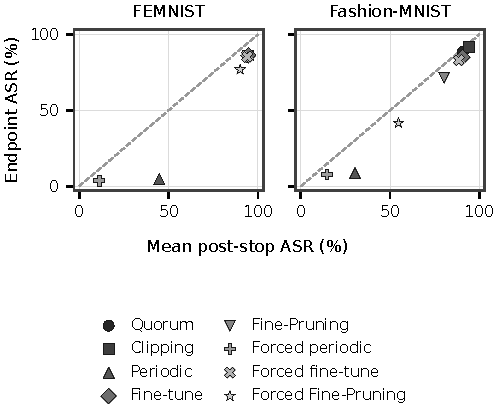
\includegraphics[width=\columnwidth]{figures/endpoint_temporal_tradeoff.pdf}
\caption{Endpoint ASR versus mean post-stop ASR. A point below the diagonal has a favorable endpoint relative to its temporal exposure.}
\label{fig:tradeoff}
\Description{Scatter plots compare endpoint and post-stop attack success across eight policies on two datasets.}
\end{figure}

\subsection{Repair phase and one-round rebound}
Table~\ref{tab:phases} separates the last repair phase from the preceding checkpoint and measures one-round changes after earlier interventions. Under continuous patch poisoning, periodic repair has mean $A_{99}=99.94\%$ on both datasets, followed by $A_{100}=7.35\%$ on FEMNIST and $12.66\%$ on Fashion-MNIST in the main comparison. After the round-50 intervention, the mean one-round increase is 42.76 percentage points on FEMNIST and 16.57 points on Fashion-MNIST. Corresponding increases after round 75 are 35.10 and 31.74 points. Thus, the endpoint advantage accompanies rapid renewed exposure at earlier intervention points.

After attacker stop, the mean round-50 changes are smaller: 1.19 points on FEMNIST and 2.73 points on Fashion-MNIST. These contrasts include all five trajectories, including rejected repairs; a scheduled intervention does not imply that a candidate was committed. They describe the deployed policy rather than the effect conditional on a successful admission.
\begin{table*}[t]
\caption{Periodic repair with the patch trigger: five-seed mean ASR at selected rounds (percent) and one-round changes after repairs (percentage points). Positive changes indicate rebound in committed ASR.}
\label{tab:phases}
\centering\small\begin{tabular}{llrrrrrrr}
\toprule
Dataset & Schedule & $A_{99}$ & $A_{100}$ & $A_{51}$ & $A_{76}$ & $A_{26}-A_{25}$ & $A_{51}-A_{50}$ & $A_{76}-A_{75}$ \\
\midrule
FEMNIST & Stop & 42.89 & 4.74 & 48.82 & 44.30 & 45.41 & 1.19 & 1.41 \\
FEMNIST & Continuous & 99.94 & 7.35 & 90.38 & 98.55 & 45.41 & 42.76 & 35.10 \\
Fashion-MNIST & Stop & 16.56 & 8.56 & 48.65 & 12.23 & 6.39 & 2.73 & 4.26 \\
Fashion-MNIST & Continuous & 99.94 & 12.66 & 81.43 & 57.97 & 6.39 & 16.57 & 31.74 \\
\bottomrule\end{tabular}
\end{table*}


\subsection{Continued poisoning and trigger transfer}
Under continuous poisoning, periodic repair has 94.62\% mean post-onset ASR on FEMNIST and 7.35\% endpoint ASR for the patch trigger. The low endpoint is measured at a scheduled repair phase. Quorum remains at 97.42\% mean post-onset ASR and 99.92\% endpoint ASR. Fine-Pruning remains at 97.24\% mean post-onset ASR and 99.94\% endpoint ASR. Fashion-MNIST also exhibits the temporal gap: in the companion comparison, periodic repair has 73.56\% mean post-onset ASR and 12.62\% endpoint ASR, while quorum has 77.35\% and 99.90\%, respectively.

The round histories in Figure~\ref{fig:rounds} show why a single endpoint is inadequate. Periodic repairs create sharp local reductions followed by rebound under future updates. Figure~\ref{fig:triggers} shows that the checkerboard trigger changes absolute rates; under continuous poisoning, periodic repair has high temporal ASR and a near-ceiling endpoint, so the low-endpoint advantage does not transfer. The transfer condition tests whether the repair bank generalizes to a spatially distinct trigger.

\begin{figure*}[t]
\centering
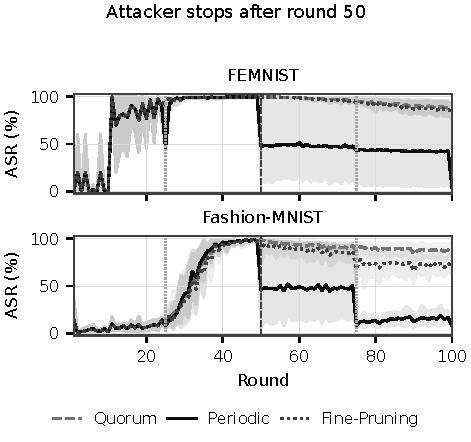
\includegraphics[width=.48\textwidth]{figures/round_trajectories_attack_stop.pdf}\hfill
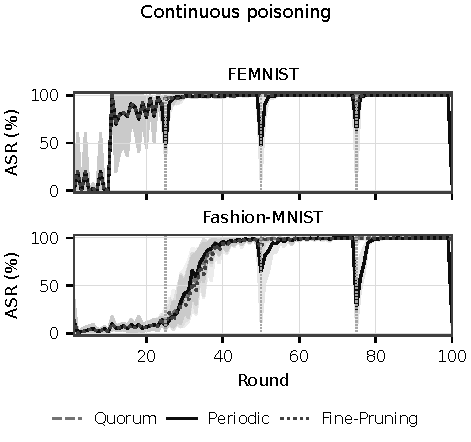
\includegraphics[width=.48\textwidth]{figures/round_trajectories_continuous.pdf}
\caption{Committed attack success over 100 rounds for quorum, periodic repair, and Fine-Pruning. Shaded bands show the 10th--90th percentile across five seed histories. Vertical dotted lines mark repair rounds; the dashed line in the left column marks attacker stop.}
\label{fig:rounds}
\Description{Round trajectories compare three defenses under attacker-stop and continuous poisoning on both datasets.}
\end{figure*}

\begin{figure}[t]
\centering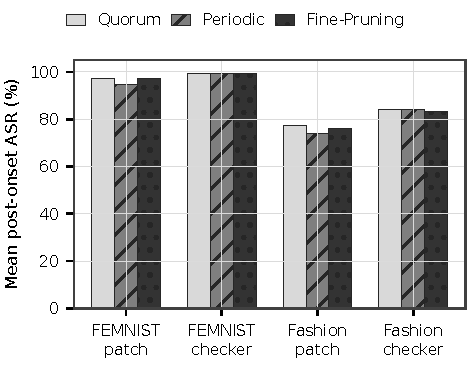
\includegraphics[width=\columnwidth]{figures/trigger_transfer_continuous.pdf}
\caption{Mean post-onset ASR under continuous poisoning for the patch and checkerboard triggers.}
\label{fig:triggers}
\Description{Grouped bars compare patch and checkerboard temporal attack success for both datasets.}
\end{figure}

\subsection{Clean utility and admission}
Clean final accuracy is similar for quorum, clipping, and private periodic repair on FEMNIST (76.57\%, 76.62\%, and 76.67\%) and Fashion-MNIST (82.43\%, 83.41\%, and 82.33\%). Forced fine-tuning and forced Fine-Pruning reduce clean accuracy relative to their private counterparts. Table~\ref{tab:stop} reports both utility and security: forced admission can lower ASR while imposing a clean-accuracy cost that the private policy would reject.

Private periodic repair admits an average of 3.0 of 4 attempts on FEMNIST and 3.6 on Fashion-MNIST in attacker-stop runs. Private Fine-Pruning admits 0.6 and 1.4 attempts, respectively. Table~\ref{tab:stop} reports these decisions directly; rejection does not by itself establish that the candidate was ineffective.

\subsection{Candidate outcomes and rejection criteria}
Table~\ref{tab:candidates} compares uncommitted candidates with the retained source model in attacked conditions. Rejected periodic candidates have lower mean ASR than their sources, whereas rejected NAD candidates have similar mean ASR. As an exploratory descriptive threshold, we count candidates that move from source ASR of at least 50\% to candidate ASR of at most 10\%. Five FEMNIST and three Fashion-MNIST periodic candidates meet this threshold while losing no more than two percentage points of test accuracy. No rejected NAD or fine-tuning candidate meets the ASR threshold. Three rejected Fashion-MNIST Fine-Pruning candidates meet it, but all lose more than two points of test accuracy. This distinction separates candidates with favorable held-out outcomes from candidates that retain the backdoor. It does not identify a rejection as incorrect under the specified private-panel rule.
\begin{table*}[t]
\caption{Rejected repairs in attacked conditions, pooled descriptively over both triggers, both schedules, and four interventions per trajectory. Source is also the retained committed model. ASR and accuracy are percentages. Strong reduction counts source ASR $\geq50\%$ and candidate ASR $\leq10\%$; the last column additionally requires a clean-accuracy loss of at most two percentage points.}
\label{tab:candidates}
\centering\small\begin{tabular}{llrrrrrrr}
\toprule
Dataset & Policy & Rejected & Source ASR & Cand. ASR & Source acc. & Cand. acc. & Strong & Utility kept \\
\midrule
FEMNIST & Periodic & 16 & 93.74 & 44.65 & 72.58 & 72.34 & 5 & 5 \\
Fashion-MNIST & Periodic & 9 & 99.69 & 42.28 & 76.23 & 76.15 & 3 & 3 \\
FEMNIST & Fine-tune & 78 & 95.14 & 93.90 & 66.49 & 66.46 & 0 & 0 \\
Fashion-MNIST & Fine-tune & 55 & 84.12 & 81.25 & 78.25 & 78.68 & 0 & 0 \\
FEMNIST & Fine-Pruning & 68 & 92.77 & 83.03 & 66.05 & 64.78 & 0 & 0 \\
Fashion-MNIST & Fine-Pruning & 56 & 78.41 & 60.39 & 78.12 & 76.65 & 3 & 0 \\
FEMNIST & NAD-style & 76 & 95.22 & 93.94 & 66.31 & 66.25 & 0 & 0 \\
Fashion-MNIST & NAD-style & 54 & 83.66 & 80.53 & 78.80 & 78.84 & 0 & 0 \\
\bottomrule\end{tabular}
\end{table*}


Table~\ref{tab:gates} counts criterion violations across both panels, counting each criterion at most once per rejected attempt. Of 167 rejected NAD candidates, 158 violate patch-loss consistency, 91 violate the accuracy tolerance, and 34 violate the clean-loss bound. For periodic repair in the main comparison, 26 of 33 rejected attempts violate the accuracy tolerance. Criteria overlap, so these counts are not a causal decomposition of rejection. Repeated quorum and periodic controls from the companion comparison are excluded from this pooled description.
\begin{table*}[t]
\caption{Private-admission decisions across clean and attacked conditions. A criterion is counted once per rejected attempt when either panel violates it. Counts overlap. Main-comparison controls are used once; NAD uses the companion comparison.}
\label{tab:gates}
\centering\small\begin{tabular}{lrrrrrr}
\toprule
Policy & Attempts & Rejected & Clean loss & Accuracy & Patch loss & Collapse \\
\midrule
Periodic & 200 & 33 & 4 & 26 & 5 & 0 \\
Fine-tune & 200 & 170 & 33 & 90 & 159 & 0 \\
Fine-Pruning & 200 & 161 & 60 & 104 & 130 & 0 \\
NAD-style & 200 & 167 & 34 & 91 & 158 & 0 \\
\bottomrule\end{tabular}
\end{table*}


The clean-training columns of Table~\ref{tab:stop} provide utility and admission references for all eight main policies. An admitted scheduled repair under clean training is an intervention count, not an attack-detection false-positive rate: the scheduler runs irrespective of attack presence.

\subsection{Repair and update-level baselines}
Table~\ref{tab:baselines} compares periodic repair, NAD-style repair, and coordinate median with quorum. Figure~\ref{fig:baseline} shows endpoint and temporal outcomes under continuous poisoning. Under attacker-stop patch poisoning, coordinate median reduces endpoint ASR to 7.89\% on FEMNIST and 2.75\% on Fashion-MNIST. Under continuous checkerboard poisoning, its endpoint ASR is 99.74\% and 75.90\%, respectively. Thus, update-level robustness also depends on the dataset and attack duration.

\begin{figure}[!htbp]
\centering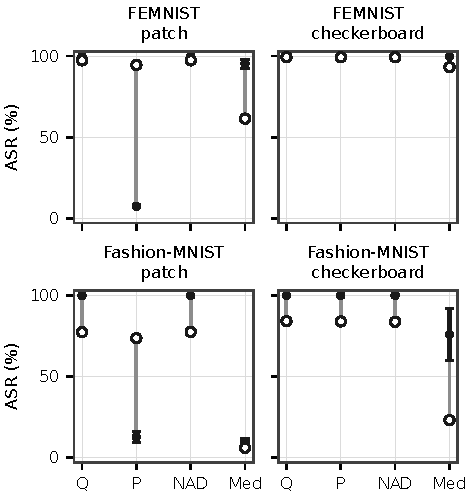
\includegraphics[width=\columnwidth]{figures/baseline_continuous.pdf}
\caption{Continuous poisoning in the companion comparison. Filled markers denote mean endpoint ASR and open markers denote mean post-onset ASR across five seeds. Lines connect the two summaries for each policy; error bars show 95\% bootstrap intervals for endpoint ASR. Q: quorum; P: periodic repair; NAD: NAD-style repair; Med: coordinate median.}
\label{fig:baseline}
\Description{Four panels compare endpoint and temporal attack success for four policies across two datasets and two triggers.}
\end{figure}

NAD-style repair is admitted in 33 of 200 attempts, compared with 168 of 200 periodic-repair attempts. In the FEMNIST patch conditions, no NAD candidate is admitted and the committed trajectory matches quorum. Rejection is therefore part of the explanation for the observed deployed outcome. Under continuous checkerboard poisoning, endpoint ASR remains approximately 100\% for both repair methods.

Coordinate median has a clean-utility cost on FEMNIST: mean clean accuracy is 69.42\%, compared with 76.57\% for quorum. On Fashion-MNIST, the corresponding means are 81.99\% and 82.43\%. Security comparisons must therefore account for the dataset-specific utility trade-off.

\begin{table*}[t]
\caption{Companion comparison: five-seed mean endpoint ASR and mean post-onset ASR (percent). Each entry is endpoint / temporal ASR. Lower values indicate less attack success.}
\label{tab:baselines}
\centering\begin{tabular}{lllrrrr}
\toprule
Dataset & Attack schedule & Trigger & Quorum & Periodic & NAD-style & Median \\
\midrule
FEMNIST & Attacker-stop & Patch & 86.15 / 94.50 & 4.74 / 65.61 & 86.15 / 94.50 & 7.89 / 23.99 \\
FEMNIST & Attacker-stop & Checkerboard & 60.07 / 89.57 & 74.01 / 89.92 & 63.46 / 90.88 & 16.31 / 59.36 \\
FEMNIST & Continuous & Patch & 99.92 / 97.42 & 7.35 / 94.62 & 99.92 / 97.42 & 95.45 / 61.42 \\
FEMNIST & Continuous & Checkerboard & 100.00 / 99.34 & 99.95 / 99.31 & 100.00 / 99.34 & 99.74 / 93.21 \\
Fashion-MNIST & Attacker-stop & Patch & 88.60 / 72.47 & 8.56 / 38.54 & 86.18 / 72.20 & 2.75 / 3.95 \\
Fashion-MNIST & Attacker-stop & Checkerboard & 85.82 / 80.10 & 80.86 / 79.10 & 77.87 / 79.47 & 4.04 / 5.90 \\
Fashion-MNIST & Continuous & Patch & 99.90 / 77.35 & 12.62 / 73.56 & 99.90 / 77.45 & 9.85 / 5.88 \\
Fashion-MNIST & Continuous & Checkerboard & 100.00 / 84.07 & 100.00 / 83.93 & 99.97 / 83.74 & 75.90 / 22.97 \\
\bottomrule\end{tabular}
\end{table*}

\subsection{Paired differences and uncertainty}
Table~\ref{tab:paired} reports paired contrasts for the patch-trigger endpoint effect and its continuous-attack and checkerboard counterparts. Comparing endpoint and post-onset differences within the same seed pair separates improvements at the final checkpoint from improvements across the deployment horizon. The checkerboard comparison retains near-ceiling endpoint ASR for periodic repair under continuous poisoning. Intervals around a difference do not establish protection when the underlying ASR remains high; they must be interpreted alongside the absolute values in Table~\ref{tab:baselines}.
\begin{table*}[t]
\caption{Paired ASR differences relative to quorum in the companion comparison (percentage points). Entries are five-seed means with pointwise 95\% bootstrap intervals. Negative values favor the listed policy.}
\label{tab:paired}
\centering\small\begin{tabular}{lllrr}
\toprule
Dataset & Condition / trigger & Policy & Endpoint difference & Post-onset difference \\
\midrule
FEMNIST & Stop / patch & Periodic & -81.41 [-88.00, -74.91] & -28.89 [-47.79, -9.98] \\
FEMNIST & Stop / patch & Median & -78.26 [-85.70, -72.04] & -70.50 [-73.51, -65.31] \\
FEMNIST & Continuous / patch & Periodic & -92.58 [-93.31, -91.63] & -2.80 [-3.47, -2.22] \\
FEMNIST & Continuous / patch & Median & -4.47 [-7.75, -1.85] & -36.00 [-39.98, -30.63] \\
FEMNIST & Continuous / checkerboard & Periodic & -0.05 [-0.16, 0.00] & -0.03 [-0.08, -0.01] \\
FEMNIST & Continuous / checkerboard & Median & -0.26 [-0.51, -0.06] & -6.14 [-9.11, -3.16] \\
Fashion-MNIST & Stop / patch & Periodic & -80.04 [-86.49, -72.78] & -33.93 [-45.37, -22.50] \\
Fashion-MNIST & Stop / patch & Median & -85.84 [-91.08, -79.32] & -68.53 [-73.53, -63.78] \\
Fashion-MNIST & Continuous / patch & Periodic & -87.27 [-90.70, -83.85] & -3.79 [-6.22, -1.37] \\
Fashion-MNIST & Continuous / patch & Median & -90.05 [-91.69, -88.58] & -71.47 [-74.69, -69.06] \\
Fashion-MNIST & Continuous / checkerboard & Periodic & 0.00 [0.00, 0.00] & -0.14 [-0.68, 0.46] \\
Fashion-MNIST & Continuous / checkerboard & Median & -24.10 [-40.25, -8.09] & -61.10 [-65.90, -55.84] \\
\bottomrule\end{tabular}
\end{table*}


\section{Discussion}
The main observation is an endpoint-temporal mismatch. A scheduled repair can produce a low ASR at the final checkpoint while most rounds in the deployment path remain exposed. Endpoint ASR describes a system deployed only after training; temporal ASR describes exposure during continued training. Metric selection therefore depends on the deployment objective.

Private admission changes the observation being made. The panel sees its reference examples and its voting rule, not the evaluation set. A rejected candidate may protect the deployment against a clean-utility loss while leaving the backdoor in place; a forced candidate may lower ASR while imposing a utility cost that the policy would normally reject. Reporting both candidate and committed outcomes is therefore necessary to identify where a result arises.

The continuous-poisoning condition combines persistent backdoor behavior with renewed malicious updates. The attacker-stop condition removes renewed poisoning after round 50. Their comparison establishes sensitivity to attack duration, while the observed differences also include the effects of admission and subsequent honest training.

\section{Limitations}
The study uses two image datasets and one small CNN lineage. Repeated Fashion-MNIST controls differed across executions, limiting exact repeatability. Fashion-MNIST has prior exposure, and FEMNIST is held out relative to prior writer partitions. The threat model assumes honest repair providers and validators, a fixed 30\% malicious fraction, model replacement, target label 0, and two trigger families. We do not evaluate adaptive attackers that optimize against the gate, corrupted providers, privacy noise, heterogeneous architectures, CIFAR-10, or network latency. Measured bytes and work describe the controller's accounting; wall-clock time and energy require deployment measurements.

\section{Conclusion}
Lifecycle evaluation changes the interpretation of repair results in federated learning. Across the main and companion comparisons, periodic repair lowers patch-trigger endpoint ASR after attacker-stop poisoning, but the mean committed ASR over later rounds remains substantially higher; under continuous poisoning the temporal mean remains high despite a favorable scheduled endpoint. Our Fine-Pruning adaptation also leaves substantial temporal exposure under its tested admission policies. These findings support reporting candidate and committed outcomes, attack exposure over a stated deployment horizon, repair admission, and post-repair continuation together.

% \clearpage
\balance
\section*{GenAI Usage Disclosure}
Generative AI tools were used strictly in an assistive capacity during the preparation of this manuscript to check grammar, improve sentence clarity, and assist with the formatting and plotting scripts for figures and tables. All AI-assisted text and visual formatting were thoroughly reviewed, verified, and edited by the authors, who take full responsibility for the accuracy and integrity of the manuscript.

\bibliographystyle{ACM-Reference-Format}
\bibliography{refs}
\end{document}
